\documentclass[14pt]{extbook}
\usepackage{multicol, enumerate, enumitem, hyperref, color, soul, setspace, parskip, fancyhdr} %General Packages
\usepackage{amssymb, amsthm, amsmath, latexsym, units, mathtools} %Math Packages
\everymath{\displaystyle} %All math in Display Style
% Packages with additional options
\usepackage[headsep=0.5cm,headheight=12pt, left=1 in,right= 1 in,top= 1 in,bottom= 1 in]{geometry}
\usepackage[usenames,dvipsnames]{xcolor}
\usepackage{dashrule}  % Package to use the command below to create lines between items
\newcommand{\litem}[1]{\item#1\hspace*{-1cm}\rule{\textwidth}{0.4pt}}
\pagestyle{fancy}
\lhead{Progress Quiz 1}
\chead{}
\rhead{Version C}
\lfoot{3629-3146}
\cfoot{}
\rfoot{Summer C 2021}
\begin{document}

\begin{enumerate}
\litem{
Write the equation of the line in the graph below in Standard Form $Ax+By=C$. Then, choose the intervals that contain $A, B, \text{ and } C$.
\begin{center}
    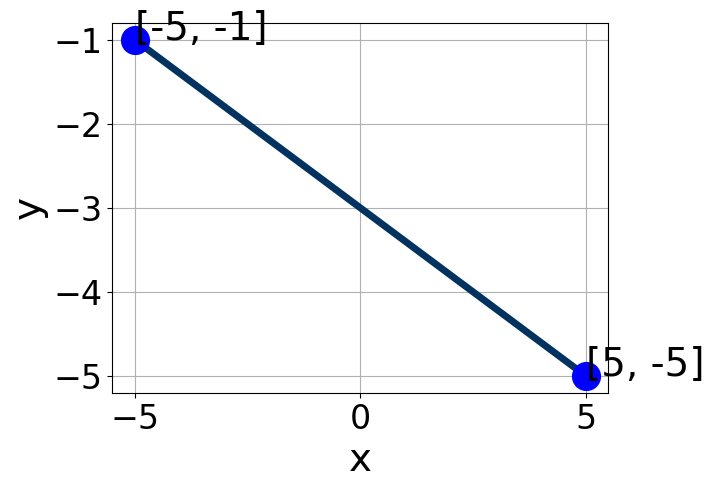
\includegraphics[width=0.5\textwidth]{../Figures/linearGraphToStandardC.png}
\end{center}
\begin{enumerate}[label=\Alph*.]
\item \( A \in [-0.5, 0.5], \hspace{3mm} B \in [-1.5, 0], \text{ and } \hspace{3mm} C \in [1, 5] \)
\item \( A \in [-4.2, -1.5], \hspace{3mm} B \in [-6.6, -3.8], \text{ and } \hspace{3mm} C \in [9, 19] \)
\item \( A \in [-0.5, 0.5], \hspace{3mm} B \in [0.2, 3.3], \text{ and } \hspace{3mm} C \in [-6, -2] \)
\item \( A \in [1.7, 2.2], \hspace{3mm} B \in [-6.6, -3.8], \text{ and } \hspace{3mm} C \in [9, 19] \)
\item \( A \in [1.7, 2.2], \hspace{3mm} B \in [3.5, 6.5], \text{ and } \hspace{3mm} C \in [-21, -13] \)

\end{enumerate} }
\litem{
Find the equation of the line described below. Write the linear equation in the form $ y=mx+b $ and choose the intervals that contain $m$ and $b$.\[ \text{Perpendicular to } 5 x - 7 y = 11 \text{ and passing through the point } (3, -9). \]\begin{enumerate}[label=\Alph*.]
\item \( m \in [-1.95, -0.92] \hspace*{3mm} b \in [-12.7, -11.3] \)
\item \( m \in [-1.95, -0.92] \hspace*{3mm} b \in [-5.4, -2.3] \)
\item \( m \in [1.19, 2.58] \hspace*{3mm} b \in [-14.4, -13.1] \)
\item \( m \in [-1.32, -0.04] \hspace*{3mm} b \in [-5.4, -2.3] \)
\item \( m \in [-1.95, -0.92] \hspace*{3mm} b \in [4.3, 7.1] \)

\end{enumerate} }
\litem{
Solve the linear equation below. Then, choose the interval that contains the solution.\[ \frac{-6x + 6}{7} - \frac{-3x + 4}{4} = \frac{4x -8}{5} \]\begin{enumerate}[label=\Alph*.]
\item \( x \in [-0.6, 1] \)
\item \( x \in [0.4, 1.9] \)
\item \( x \in [10.4, 12.3] \)
\item \( x \in [2.4, 4] \)
\item \( \text{There are no real solutions.} \)

\end{enumerate} }
\litem{
Write the equation of the line in the graph below in Standard Form $Ax+By=C$. Then, choose the intervals that contain $A, B, \text{ and } C$.
\begin{center}
    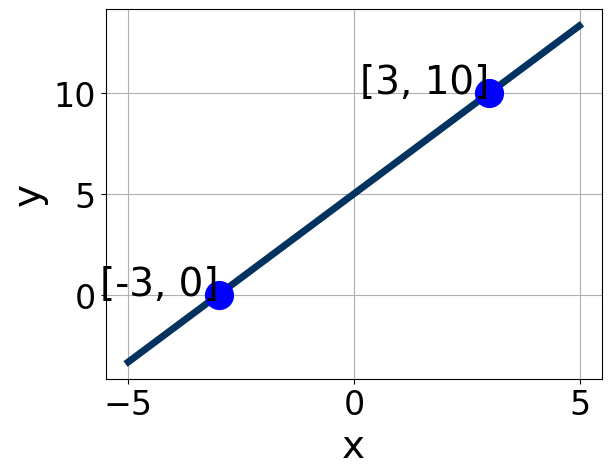
\includegraphics[width=0.5\textwidth]{../Figures/linearGraphToStandardCopyC.png}
\end{center}
\begin{enumerate}[label=\Alph*.]
\item \( A \in [-3, 0.3], \hspace{3mm} B \in [-0.5, 2.4], \text{ and } \hspace{3mm} C \in [0, 12] \)
\item \( A \in [-8.2, -1.7], \hspace{3mm} B \in [2.9, 3.9], \text{ and } \hspace{3mm} C \in [15, 26] \)
\item \( A \in [2.4, 5.7], \hspace{3mm} B \in [-3.7, -2.4], \text{ and } \hspace{3mm} C \in [-15, -13] \)
\item \( A \in [2.4, 5.7], \hspace{3mm} B \in [2.9, 3.9], \text{ and } \hspace{3mm} C \in [15, 26] \)
\item \( A \in [-3, 0.3], \hspace{3mm} B \in [-2.2, -0.9], \text{ and } \hspace{3mm} C \in [-8, -3] \)

\end{enumerate} }
\litem{
Find the equation of the line described below. Write the linear equation in the form $ y=mx+b $ and choose the intervals that contain $m$ and $b$.\[ \text{Parallel to } 9 x - 8 y = 7 \text{ and passing through the point } (-3, -5). \]\begin{enumerate}[label=\Alph*.]
\item \( m \in [1.01, 1.38] \hspace*{3mm} b \in [1.53, 1.73] \)
\item \( m \in [1.01, 1.38] \hspace*{3mm} b \in [-1.96, -1.53] \)
\item \( m \in [1.01, 1.38] \hspace*{3mm} b \in [-2.13, -1.8] \)
\item \( m \in [-0.45, 1.02] \hspace*{3mm} b \in [-1.96, -1.53] \)
\item \( m \in [-1.49, 0.54] \hspace*{3mm} b \in [-8.58, -8.29] \)

\end{enumerate} }
\litem{
Solve the linear equation below. Then, choose the interval that contains the solution.\[ \frac{-3x + 8}{3} - \frac{8x -9}{7} = \frac{-3x -9}{5} \]\begin{enumerate}[label=\Alph*.]
\item \( x \in [2.73, 5.73] \)
\item \( x \in [-1.28, 1.72] \)
\item \( x \in [1.06, 3.06] \)
\item \( x \in [15.85, 18.85] \)
\item \( \text{There are no real solutions.} \)

\end{enumerate} }
\litem{
First, find the equation of the line containing the two points below. Then, write the equation in the form $ y=mx+b $ and choose the intervals that contain $m$ and $b$.\[ (-4, -3) \text{ and } (8, -9) \]\begin{enumerate}[label=\Alph*.]
\item \( m \in [-0.54, 0.07] \hspace*{3mm} b \in [-8, -4] \)
\item \( m \in [0.44, 0.55] \hspace*{3mm} b \in [-13, -12] \)
\item \( m \in [-0.54, 0.07] \hspace*{3mm} b \in [-17, -15] \)
\item \( m \in [-0.54, 0.07] \hspace*{3mm} b \in [5, 7] \)
\item \( m \in [-0.54, 0.07] \hspace*{3mm} b \in [-3, 2] \)

\end{enumerate} }
\litem{
Solve the equation below. Then, choose the interval that contains the solution.\[ -15(-3x + 5) = -17(-19x + 11) \]\begin{enumerate}[label=\Alph*.]
\item \( x \in [0.79, 1.37] \)
\item \( x \in [0.05, 0.69] \)
\item \( x \in [-1.11, -0.94] \)
\item \( x \in [0.57, 0.93] \)
\item \( \text{There are no real solutions.} \)

\end{enumerate} }
\litem{
First, find the equation of the line containing the two points below. Then, write the equation in the form $ y=mx+b $ and choose the intervals that contain $m$ and $b$.\[ (-3, 9) \text{ and } (8, 2) \]\begin{enumerate}[label=\Alph*.]
\item \( m \in [-2.49, 0.19] \hspace*{3mm} b \in [10.07, 12.91] \)
\item \( m \in [0.47, 2.35] \hspace*{3mm} b \in [-3.67, -2.56] \)
\item \( m \in [-2.49, 0.19] \hspace*{3mm} b \in [-6.04, -5.31] \)
\item \( m \in [-2.49, 0.19] \hspace*{3mm} b \in [-7.21, -6.31] \)
\item \( m \in [-2.49, 0.19] \hspace*{3mm} b \in [6.55, 7.96] \)

\end{enumerate} }
\litem{
Solve the equation below. Then, choose the interval that contains the solution.\[ -15(13x + 14) = -12(-5x -16) \]\begin{enumerate}[label=\Alph*.]
\item \( x \in [-0.25, -0.11] \)
\item \( x \in [-0.12, -0.05] \)
\item \( x \in [-1.67, -1.46] \)
\item \( x \in [0.01, 0.09] \)
\item \( \text{There are no real solutions.} \)

\end{enumerate} }
\end{enumerate}

\end{document}